%FILE FOR RISK ANALYSIS
There are many risks and reasons why a project might fail or go bad, A change in organizational priorities is the most common reason. A change in project objectives is also common as poor communication and unclear risk definition.
	\begin{itemize}
		\setlength\itemsep{-0.2em}
		\item Unclear or shifting goals.
		\item lack of planning.
		\item lack of follow up.
		\item timing issues 
		\item Lack of risk management.
		\item Unsuitable tools.
		\item Too many unsuitable tools
	\end{itemize}

For these reasons and many more, we’ve created an overall table with ratings which rate the opportunity/effect and risk.

\subsubsection{Scale} %SMALL HEADER
Ratings that can be seen below are from 1 to 9. Where 1 is low risk and 9 is high risk.\\
	
	\begin{figure}[!ht]
		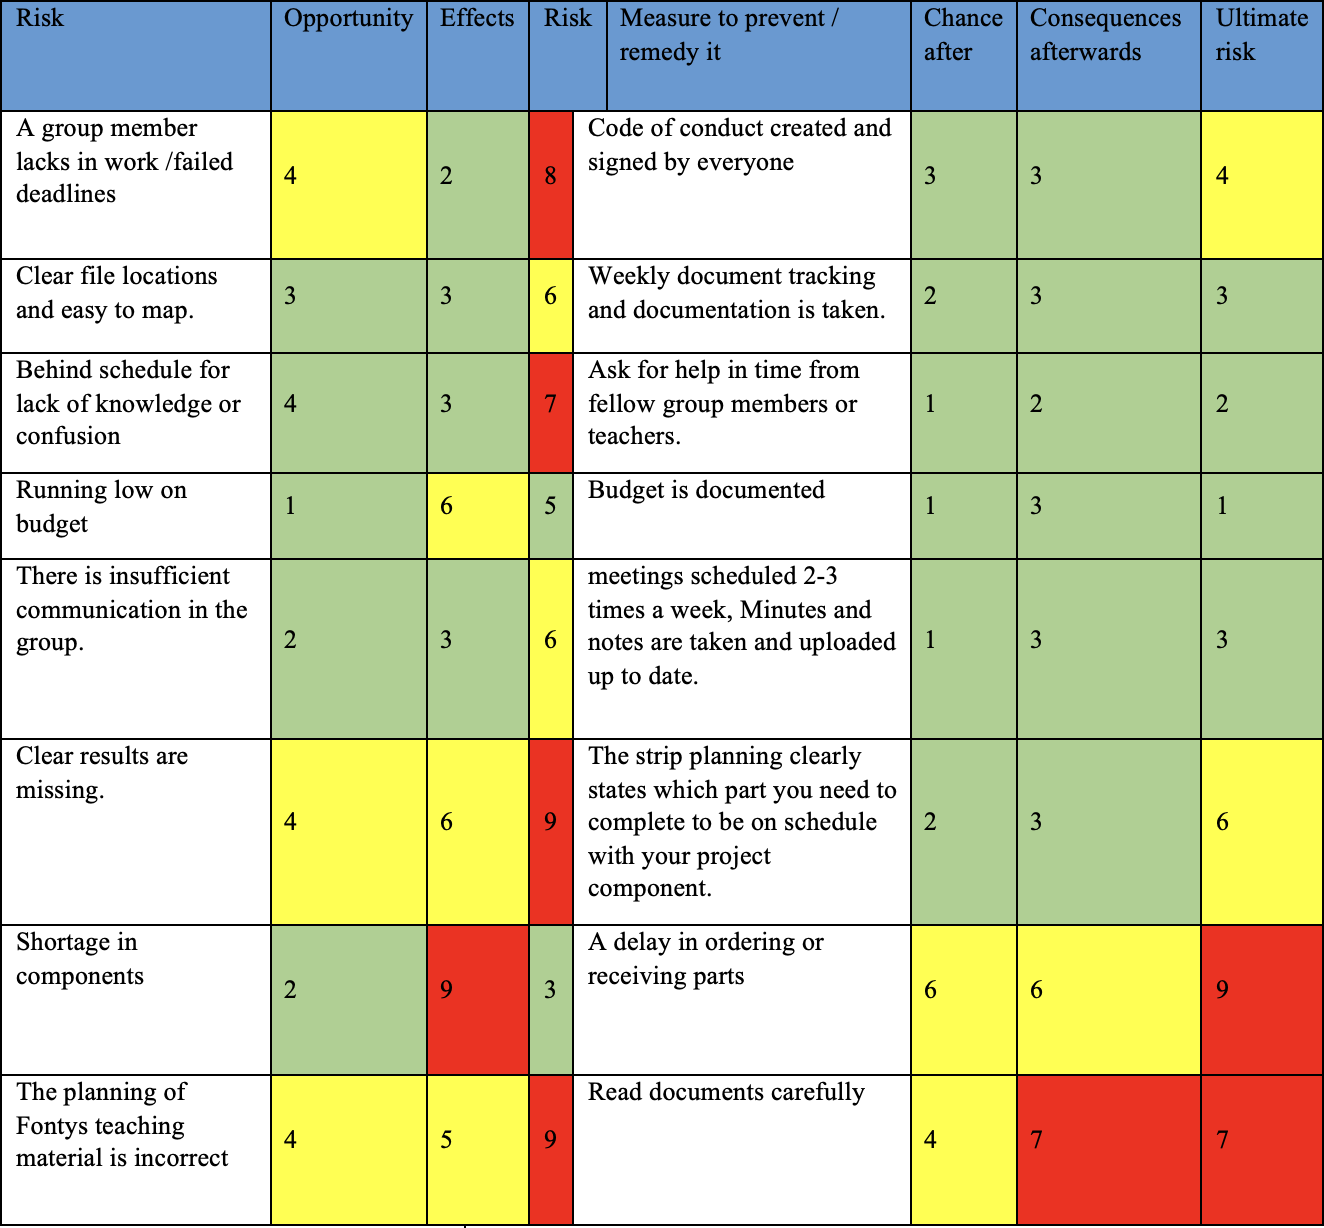
\includegraphics[scale = 0.4]{risk}
		\caption{Table with risk rating}
		\label{fig:risk}
	\end{figure}